%%%%%%%%%%%%%%%%%%%%%%%%%%%%%%%%%%%%%%%%%%%%%%%%%%%%%%%%%%%%%%%%%%%%%%%%%%%%%%%%
%%%%%%%%%%%%%%%%%%%%%%%%%%%%%%%%%%%%%%%%%%%%%%%%%%%%%%%%%%%%%%%%%%%%%%%%%%%%%%%%
%%%%%%%%%%%%%%%%%%%%%%%%%%%%%%%%%%%%%%%%%%%%%%%%%%%%%%%%%%%%%%%%%%%%%%%%%%%%%%%%
\section{Regressão}

\index{Regressão}

\begin{wrapfigure}{l}{0.5\textwidth}
     \centering
     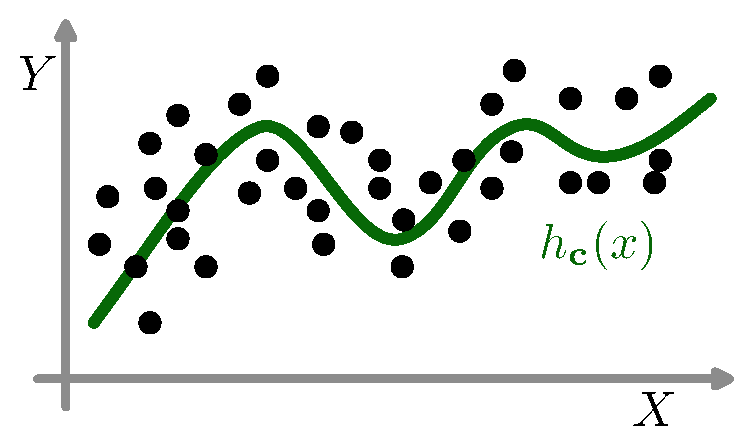
\includegraphics[width=0.45\textwidth]{chapters/notacao/regressao1.eps}
     \caption{Regressão de uma curva $h_{\VECTOR{c}}(x)$ com parâmetros $\VECTOR{c}$ num conjunto de dados. }
     \label{fig:regressao:1}
    \hspace{20pt}
\end{wrapfigure}
A regressão é o processo pelo qual uma curva ou superfície em múltiplas dimensões é 
ajustada num conjunto de dados, quando se sabe ou se aceita que existirá um erro no ajuste
devido à natureza ruidosa dos dados \cite[pp. 5]{chapra2016metodos}.

A ideia geral da regressão é achar uma curva de ajuste que represente melhor 
os dados, sem que a curva necessariamente coincida de forma exata com todos eles,
pelo que devemos definir algum critério de medida do erro de ajuste 
e procurar uma curva que minimize esse erro \cite[pp. 7]{chapra2016metodos}.

Assim, a regressão pode ser classificada mediante o tipo de curva de ajuste que é usado;
nesse sentido, podemos verificar na literatura:

\begin{itemize}
\item \textbf{Regressão linear}: 
Este caso ocorre quando usamos uma linha reta;
sendo esta uma função $h_{\VECTOR{c}}:\mathbb{R} \rightarrow \mathbb{R}$ de parâmetros $\VECTOR{c}$, 
utilizada para aproximar um conjunto de dados \cite[pp. 398, 402]{chapra2016metodos} \cite[pp. 25]{aster2013parameter}.
A regressão linear é um caso particular da regressão polinomial quando $M=1$.
\begin{example}~
\begin{itemize}
\item Curva de ajuste na regressão linear, 
\begin{equation}
h_{\VECTOR{c}}(x)=c_1+c_2 x.
\end{equation}
\item Na Seção \ref{sec:theo:reglogr1r1:1}, após uma linearização de uma relação não linear,
como na função logística, podemos ver exemplos de regressão linear.
\end{itemize}
\end{example}

\item \textbf{Regressão polinomial}: 
Indica que usamos um polinômio de grau $M$,
sendo esta uma função $h_{\VECTOR{c}}:\mathbb{R} \rightarrow \mathbb{R}$ com parâmetros $\VECTOR{c}$, 
utilizada para aproximar um conjunto de dados \cite[pp. 399, 415]{chapra2016metodos}.
\begin{example}~
\begin{itemize}
\item Curva de ajuste na regressão polinomial com grau $M=2$,
\begin{equation}
h_{\VECTOR{c}}(x)=c_1+c_2 x+c_3 x^2.
\end{equation}
\item Na Seção \ref{sec:theo:maphxr1r1}, podemos ver exemplos de regressão polinomial.
\item Na Seção \ref{sec:theo:reglogr1r1poly:1} após uma linearização de uma relação não linear,
como na função logística, podemos ver exemplos de regressão polinomial.
\end{itemize}
\end{example}

\item \textbf{Regressão não linear}: 
Neste caso, usamos um ajuste de dados
com uma função $h_{\VECTOR{c}}:\mathbb{R} \rightarrow \mathbb{R}$ com parâmetros $\VECTOR{c}$, 
que representa uma relação não linear entre o domínio e o contradomínio de $h_{\VECTOR{c}}$ 
\cite[pp. 424]{chapra2016metodos} \cite[pp. 217]{agarwal2014creators}.
\begin{example}~
\begin{itemize}
\item Um caso de curva de ajuste na regressão não linear, 
\begin{equation}
h_{\VECTOR{c}}(x)=c_1 e^{-c_2 x}.
\end{equation}
\item Na Seção \ref{sec:theo:maphcxr1r1}, podemos ver exemplos de regressão não linear.
\end{itemize}
\end{example}

\item \textbf{Regressão linear múltipla}:
Temos este caso quando ajustamos um hiperplano;
sendo esta uma função $h_{\VECTOR{c}}:\mathbb{R}^{N} \rightarrow \mathbb{R}$ com parâmetros $\VECTOR{c}$, 
utilizada para aproximar um conjunto de dados \cite[pp. 399, 418]{chapra2016metodos}.
A regressão linear é um caso particular da regressão linear múltipla quando $N=1$.
\begin{example}~
\begin{itemize}
\item Curva de ajuste na regressão linear múltipla com $N=2$, 
\begin{equation}
h_{\VECTOR{c}}(\VECTOR{x})=c_1+c_2 x_1+c_3 x_2.
\end{equation}
\item Na Seção \ref{sec:theo:reglogrnr1:1}, após uma linearização de uma relação não linear,
como na função logística, podemos ver exemplos de regressão linear múltipla.
\end{itemize}
\end{example}

\item \textbf{Regressão polinomial múltipla}:
Acontece quando ajustamos um polinômio multivariado de grau total $M$,
sendo esta uma função $h_{\VECTOR{c}}:\mathbb{R}^{N} \rightarrow \mathbb{R}$ com parâmetros $\VECTOR{c}$, 
utilizada para aproximar um conjunto de dados.
A regressão polinomial é um caso particular da regressão polinomial múltipla quando $N=1$.
\begin{example}~
\begin{itemize}
\item Um caso de curva de ajuste na regressão polinomial múltipla com 
$N=2$ e $h_{\VECTOR{c}}:\mathbb{R}^{2} \rightarrow \mathbb{R}$, 
\begin{equation}
h_{\VECTOR{c}}(\VECTOR{x})=c_1+c_2 x_1+c_3 x_2+c_4 x_1^2+c_5 x_2^2+c_6 x_1 x_2.
\end{equation}
\item Nas Seções \ref{sec:theo:maphxr2r1} e \ref{sec:theo:maphxr2r2},
 podemos ver exemplos de regressão polinomial múltipla.
\item Na Seção \ref{sec:theo:reglogrnr1poly:1}, após uma linearização de uma relação não linear,
como na função logística, podemos ver exemplos de regressão polinomial múltipla.
\end{itemize}
\end{example}

\item \textbf{Regressão não linear múltipla}: 
Estamos neste caso quado usamos no ajuste dos dados
uma função $h_{\VECTOR{c}}:\mathbb{R}^{N} \rightarrow \mathbb{R}$, 
que representa uma função não linear entre o domínio e o contradomínio de $h_{\VECTOR{c}}$.
A regressão não linear é um caso particular da regressão não linear múltipla quando $N=1$.
\begin{example}~
\begin{itemize}
\item Um caso de curva de ajuste na regressão não linear múltipla, 
\begin{equation}
h_{\VECTOR{c}}(\VECTOR{x})=c_1 e^{- c_2^2(x_1 -c_3)^2- c_4^2(x_2 -c_5)^2}.
\end{equation}
\item Na Seção \ref{sec:theo:maphcxrnr1}, podemos ver exemplos de regressão não linear múltipla.
\item Na Seção \ref{sec:theo:reglogrnr1nolinear:1}, após uma linearização de uma relação não linear,
como na função logística, podemos ver exemplos de regressão não linear múltipla.
\end{itemize}
\end{example}
\end{itemize}

\subsection{Linearização de curvas de ajuste não lineares}

Os problemas de \textbf{regressão não linear}
em alguns casos podem ser modificados para ter a forma de um 
problema de \textbf{regressão linear} (simples ou múltipla);
essa caraterística é interessante, pois geralmente
os problemas não lineares são resolvidos com métodos iterativos,
que podem ou não convergir na solução.
Em contrapartida, em problemas de regressão linear,
os métodos disponíveis nos brindam com uma resposta mediante um procedimento 
predeterminado, 
o que facilita o planejamento de um procedimento de solução e favorece o tempo de computo.

Assim, na continuação mostramos 
como problemas não lineares podem ser 
adaptados a um problema de regressão linear (simples):
\begin{example}
Usando 
$\hat{y}=ln(y)$,  
$\hat{x}=ln(x)$, 
$\hat{c}_1=ln(c_1)$, e
$\hat{c}_2=c_2$, obtemos %$\hat{y}=\hat{c}_1+\hat{c}_2 \hat{x}$.
\begin{equation}
y=c_1x^{c_2}
\quad \rightarrow \quad 
\hat{y}=\hat{c}_1+\hat{c}_2 \hat{x}.
\end{equation}
\vspace{-2pt}
\end{example}

\begin{example}%[Curva de ajuste $y=c_1 {c_2}^x$:]
Usando 
$\hat{y}=ln(y)$,  
$\hat{x}=x$, 
$\hat{c}_1=ln(c_1)$, e
$\hat{c}_2=ln(c_2)$, obtemos %$\hat{y}=\hat{c}_1+\hat{c}_2 \hat{x}$.
\begin{equation}
y=c_1 {c_2}^x
\quad \rightarrow \quad 
\hat{y}=\hat{c}_1+\hat{c}_2 \hat{x}.
\end{equation}
\vspace{-2pt}
\end{example}

\begin{example}%[Curva de ajuste $y=\left(c_1 + {c_2} x \right)^{-1}$:]
Usando 
$\hat{y}=\frac{1}{y}$,  
$\hat{x}=x$, 
$\hat{c}_1=c_1$, e 
$\hat{c}_2=c_2$, obtemos %$\hat{y}=\hat{c}_1+\hat{c}_2 \hat{x}$.
\begin{equation}
y=\left(c_1 + {c_2} x \right)^{-1}
\quad \rightarrow \quad 
\hat{y}=\hat{c}_1+\hat{c}_2 \hat{x}.
\end{equation}
\vspace{-2pt}
\end{example}

\begin{example}%[Curva de ajuste $y=c_1 x \left(c_2 + x\right)^{-1}$:] 
Usando 
$\hat{y}=\frac{1}{y}$,  
$\hat{x}=\frac{1}{x}$, 
$\hat{c}_1=\frac{1}{c_1}$, e 
$\hat{c}_2=\frac{c_2}{c_1}$, obtemos %$\hat{y}=\hat{c}_1+\hat{c}_2 \hat{x}$.
\begin{equation}
y=c_1 x \left(c_2 + x\right)^{-1}
\quad \rightarrow \quad 
\hat{y}=\hat{c}_1+\hat{c}_2 \hat{x}.
\end{equation}
\vspace{-2pt}
\end{example}

De forma similar ao caso de regressão linear simples,
curvas de ajuste não lineares podem ser adaptadas a um problema de regressão linear múltipla:
\begin{example}%[Curva de ajuste $y=c_1 +c_2 x + c_3 x^2 + c_4 x^3$:]
Usando 
$\hat{y}=y$,  
$\hat{x}_1=x$,
$\hat{x}_2=x^2$,
$\hat{x}_3=x^3$, 
$\hat{c}_1=c_1$, 
$\hat{c}_2=c_2$, 
$\hat{c}_3=c_3$, e 
$\hat{c}_4=c_4$, obtemos %$\hat{y}=\hat{c}_1+\hat{c}_2 \hat{x}_1+\hat{c}_2 \hat{x}_2+\hat{c}_3 \hat{x}_3$.
\begin{equation}
y=c_1 +c_2 x + c_3 x^2 + c_4 x^3
\quad \rightarrow \quad 
\hat{y}=\hat{c}_1+\hat{c}_2 \hat{x}_1+\hat{c}_2 \hat{x}_2+\hat{c}_3 \hat{x}_3.
\end{equation}
\vspace{-2pt}
\end{example}

\begin{example}%[Curva de ajuste $y=c_1 +c_2 \sqrt{x} + c_3 sin(x)$:]
Usando 
$\hat{y}=y$,  
$\hat{x}_1=\sqrt{x}$,
$\hat{x}_2=sin(x)$, 
$\hat{c}_1=c_1$, 
$\hat{c}_2=c_2$, e 
$\hat{c}_3=c_3$, obtemos %$\hat{y}=\hat{c}_1+\hat{c}_2 \hat{x}_1+\hat{c}_2 \hat{x}_2$.
\begin{equation}
y=c_1 +c_2 \sqrt{x} + c_3 sin(x)
\quad \rightarrow \quad 
\hat{y}=\hat{c}_1+\hat{c}_2 \hat{x}_1+\hat{c}_2 \hat{x}_2.
\end{equation}
\vspace{-2pt}
\end{example}
